\begin{figure}[!htbp]
  \centering
  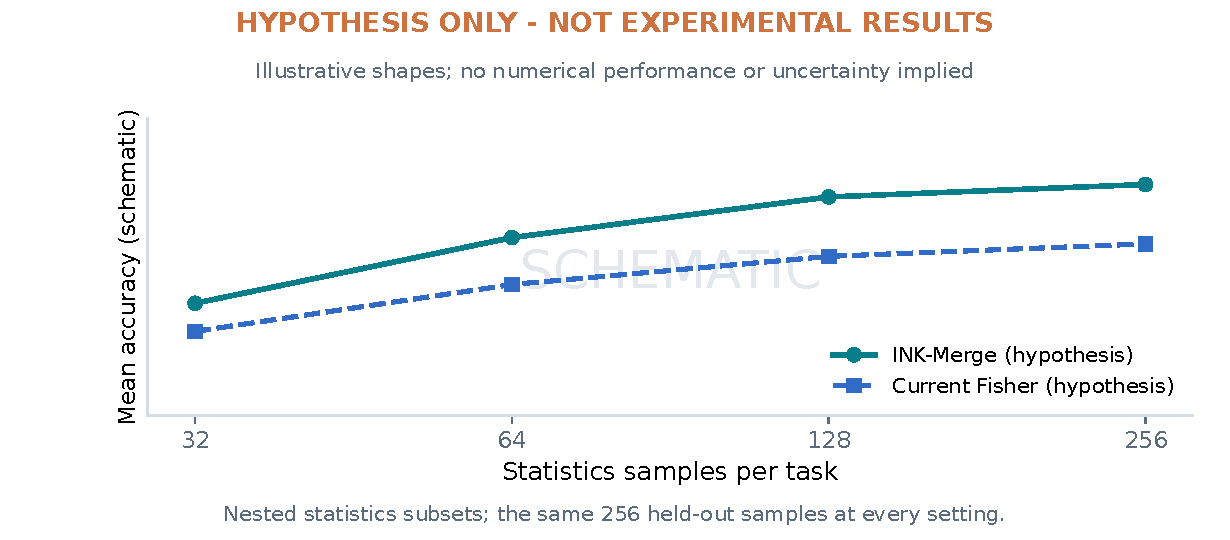
\includegraphics[width=0.78\linewidth]{figures/hypothesis_samples.pdf}
  \caption{\textbf{统计样本量的预期趋势示意，非实验结果。}待验证假设是样本增加带来收益递减，修正几何可能在有限样本下优于当前 Fisher。曲线间距和拐点仅供解释，既不是测得的性能差值，也不证明 128 或 256 个样本已经足够。}
  \label{fig:ink-sample-size-analysis}
\end{figure}
